\documentclass{article}
\usepackage{amsmath}
\usepackage{graphicx}
\usepackage[a4paper, margin=1in]{geometry}
\usepackage{pgfplots}
\pgfplotsset{compat=1.17}
\usepackage{afterpage}
\usepackage{float}
\usepackage{hyperref}
\usepackage{subcaption}
\graphicspath{{assets/}}

\title{Parallel sorting of large arrays using Bitonic Sort in CUDA}
\author{Epameinondas Bakoulas}
\date{February 2025}

\begin{document}

\maketitle

\section{Objective}
Sorting algorithms usually take $O(nlogn)$ time to sort an array of size n. Bitonic sort is a parallel sorting 
algorithm that can sort very large arrays faster. By leveraging the power of modern GPUs we can achieve a noticeable
speedup compared to CPU sorting algorithms, either single threaded or multi threaded.

\section{Algorithm Analysis}

\subsection{Overview}

Our goal is to sort an array of size $2^q$, where $q = [15:28]$. We will present a total of 3 implementation, V0, V1 and V2.
The first implementation, V0, is a simple implementation of the algorithm that is noticeably slower than the other two.

\subsection{Algorithm implementation in CUDA (V0)}

The algorithm will follow the standard \textbf{Bitonic Sort Network} pattern as shown in Figure \ref{fig:bitonic-sort-network}.
Our goal is to create bitonic sequences of size $2, 4, 8, ..., p$ and then, with the correct exchanges between
processes, make bigger bitonic sequences. 
The main logic of the algorithm is shown in Figure \ref{alg:bitonic-sort}.
The variable \texttt{group\_size} is the size of the bitonic sequence that we
create in each iteration. On every iteration, we double the size of \texttt{group\_size} to create bigger bitonic sequences.

The variable \texttt{distance} is the distance between the elements that we compare in each iteration. We start with
\texttt{group\_size/2} and we divide it by 2 in each iteration. This way, we compare the elements of the bitonic sequence
in a specific order, as shown in Figure \ref{fig:bitonic-sort-network}.

For each \texttt{group\_size} we need to perform $\log_2{\texttt{group\_size}}$ iterations. For example, if we have 8
elements in each group, we need to perform 3 iterations with a specific distance each time.

The kernel function \texttt{exchange} is responsible for exchanging the elements of the bitonic sequence. Before we run it,
we need to specify the number of blocks and threads (in each block) that we will use. Since we're performing $n/2$ exchanges
in each iteration, we need to have \textbf{n/2} \textbf{threads in total}. We will use the max number of threads allowed in each block, which
is 1024. This means that we need to have $\mathbf{\frac{n/2}{1024}}$ \textbf{blocks in total}.

Each thread inside the kernel function is responsible for exchanging two elements of the bitonic sequence. It needs to
compute the following things:
\begin{enumerate}
    \item Who am I? What's my thread ID?
    \item What's the index of the element that I'm going to work with?
    \item What's the index of the element that I'm going to compare with?
    \item Which index should keep to minimum and which the maximum?
\end{enumerate}

The answers to those questions can be found in Figure \ref{fig:exchange-kernel}. The method of finding the partner is
explain later on in detail with the hypercube model.

\begin{figure}[H]
    \centering
    \includegraphics[width=1\textwidth]{bitonic_sort.png}
    \caption{Bitonic Sort Algorithm}
    \label{alg:bitonic-sort}
\end{figure}


\begin{figure}[H]
    \centering
    \includegraphics[width=1\textwidth]{bitonic-sort-network.png}
    \caption{Bitonic Sort Network. The arrow points to the element that keeps the maximum.}
    \label{fig:bitonic-sort-network}
\end{figure}

\begin{figure}[H]
    \centering
    \includegraphics[width=1\textwidth]{exchange-v0.png}
    \caption{Exchange Kernel function. Each thread is responsible for only one exchange.}
    \label{fig:exchange-kernel}
\end{figure}


\subsection{Hypercube model}

Finding the right partner to exchange data with in each stage of the algorithm can be quite tricky. One possible way
is to leverage the power of the hypercube model. The index of the element that we're going to exchange with can be
found by performing a bitwise XOR operation between the current index and the distance:
$$i \oplus distance$$

In Figure \ref{fig:hypercube-model} we can see the exchanges performed between 8 elements.

\begin{figure}[h]
    \centering
    
    \begin{subfigure}[b]{0.45\textwidth}
        \centering
        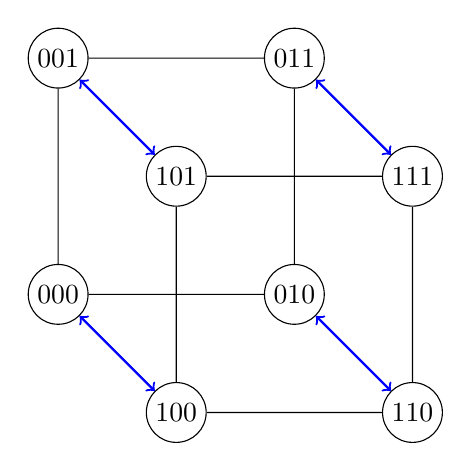
\begin{tikzpicture}[scale=1.5, every node/.style={circle, draw, fill=white, inner sep=2pt, text centered}]
            % 1st Cube (Upper Left)
            \node (3D-1) at (1,-3.5) {000};
            \node (3D-2) at (1,-1.5) {001};
            \node (3D-3) at (3,-3.5) {010};
            \node (3D-4) at (3,-1.5) {011};
            \node (3D-5) at (2,-4.5) {100};
            \node (3D-6) at (2,-2.5) {101};
            \node (3D-7) at (4,-4.5) {110};
            \node (3D-8) at (4,-2.5) {111};
            
            % Edges for the first cube (Upper Left)
            \draw (3D-1) -- (3D-2);
            \draw (3D-2) -- (3D-4);
            \draw (3D-4) -- (3D-3);
            \draw (3D-3) -- (3D-1);
            \draw [<->, thick, draw=blue] (3D-1) -- (3D-5);
            \draw [<->, thick, draw=blue] (3D-2) -- (3D-6);
            \draw [<->, thick, draw=blue] (3D-3) -- (3D-7);
            \draw [<->, thick, draw=blue] (3D-4) -- (3D-8);
            \draw (3D-5) -- (3D-6);
            \draw (3D-6) -- (3D-8);
            \draw (3D-8) -- (3D-7);
            \draw (3D-7) -- (3D-5);
        \end{tikzpicture}
        \caption{Exchanges at distance 4}
    \end{subfigure}
    \hfill
    \begin{subfigure}[b]{0.45\textwidth}
        \centering
        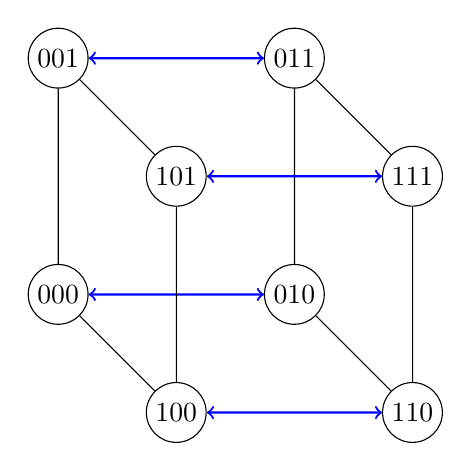
\begin{tikzpicture}[scale=1.5, every node/.style={circle, draw, fill=white, inner sep=2pt, text centered}]
            % 2nd Cube (Upper Right)
            \node (3D-9) at (6,-3.5) {000};
            \node (3D-10) at (6,-1.5) {001};
            \node (3D-11) at (8,-3.5) {010};
            \node (3D-12) at (8,-1.5) {011};
            \node (3D-13) at (7,-4.5) {100};
            \node (3D-14) at (7,-2.5) {101};
            \node (3D-15) at (9,-4.5) {110};
            \node (3D-16) at (9,-2.5) {111};
            
            % Edges for the second cube (Upper Right)
            \draw (3D-9) -- (3D-10);
            \draw[<->, thick, draw=blue] (3D-10) -- (3D-12);
            \draw (3D-12) -- (3D-11);
            \draw[<->, thick, draw=blue] (3D-11) -- (3D-9);
            \draw (3D-9) -- (3D-13);
            \draw (3D-10) -- (3D-14);
            \draw (3D-11) -- (3D-15);
            \draw (3D-12) -- (3D-16);
            \draw (3D-13) -- (3D-14);
            \draw[<->, thick, draw=blue] (3D-14) -- (3D-16);
            \draw (3D-16) -- (3D-15);
            \draw[<->, thick, draw=blue] (3D-15) -- (3D-13);
        \end{tikzpicture}
        \caption{Exchanges at distance 2}
    \end{subfigure}
    \hfill
    \begin{subfigure}[b]{0.6\textwidth}
        \centering
        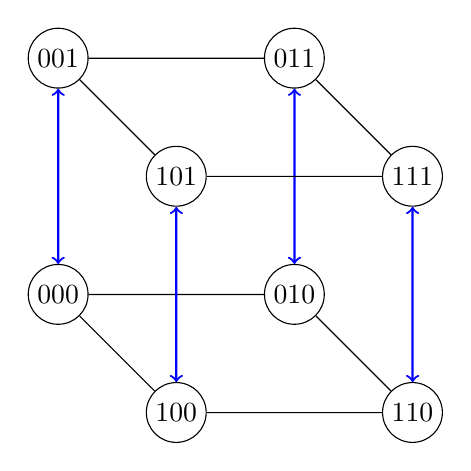
\begin{tikzpicture}[scale=1.5, every node/.style={circle, draw, fill=white, inner sep=2pt, text centered}]
            % 3rd Cube (Lower Middle)
            \node (3D-17) at (4,-7.5) {000};
            \node (3D-18) at (4,-5.5) {001};
            \node (3D-19) at (6,-7.5) {010};
            \node (3D-20) at (6,-5.5) {011};
            \node (3D-21) at (5,-8.5) {100};
            \node (3D-22) at (5,-6.5) {101};
            \node (3D-23) at (7,-8.5) {110};
            \node (3D-24) at (7,-6.5) {111};
            
            % Edges for the third cube (Lower Middle)
            \draw[<->, thick, draw=blue] (3D-17) -- (3D-18);
            \draw (3D-18) -- (3D-20);
            \draw[<->, thick, draw=blue] (3D-20) -- (3D-19);
            \draw (3D-19) -- (3D-17);
            \draw (3D-17) -- (3D-21);
            \draw (3D-18) -- (3D-22);
            \draw (3D-19) -- (3D-23);
            \draw (3D-20) -- (3D-24);
            \draw[<->, thick, draw=blue] (3D-21) -- (3D-22);
            \draw (3D-22) -- (3D-24);
            \draw[<->, thick, draw=blue] (3D-24) -- (3D-23);
            \draw (3D-23) -- (3D-21);
        \end{tikzpicture}
        \caption{Exchanges at distance 1}
    \end{subfigure}
    
    \caption{(Hyper)cube model with 8 processes.}
    \label{fig:hypercube-model}
\end{figure}

\subsection{Minimizing the kernel calls (V1)}

In the previous implementation, we had to call the kernel function \texttt{exchange} for each exchange. This is necessary
if we want to achieve synchonization. However, we can leverage the fact that threads inside a block can synchronize with each
other. This means that all 1024 threads inside the block can be synchronized.

For the V1 implementation, we will create 2 new kernel functions \texttt{initialExchangeLocally} and \texttt{exchangeLocally}.
The first one will be responsible for the initial exchanges at the start of the algorithm, up until we reach $group\_size = 2048$.
This means that all of the exchanges with $distance <= 1024$ will be performed in a \textbf{single kernel call}. After that, we 
will call the same V0 kernel function up until we reach $distance = 1024$, where we will call the \texttt{exchangeLocally} function.

The 2 new functions might seem similar, but they have a key difference. The \texttt{initialExchangeLocally} function will increase
the \texttt{group\_size} by 2 in each iteration, while the \texttt{exchangeLocally} function runs on a specific \texttt{group\_size} value. 
The code is shown in Figures \ref{alg:bitonic-sort-v1} and \ref{alg:initial-exchange-locally-v1}.

\begin{figure}[H]
    \centering
    \includegraphics[width=1\textwidth]{bitonic_sort_v1.png}
    \caption{Bitonic Sort Algorithm, modified to perform less amount of kernel calls (V1)}
    \label{alg:bitonic-sort-v1}
\end{figure}

\begin{figure}[H]
    \centering
    \includegraphics[width=1\textwidth]{initial-exchange-locally-v1.png}
    \caption{Initial exchanges performed at the start of the algorithm (V1)}
    \label{alg:initial-exchange-locally-v1}
\end{figure}

\subsection{From Global memory to Shared (V2)}
We can further optimize the algorithm by using shared memory. Generally, shared memory has 100x faster access time than global memory.
The V2 implementation will use shared memory inside the functions \texttt{initialExchangeLocally} and \texttt{exchangeLocally}.

First, we need to transfer the data from the global memory to the shared memory. Each thread will be responsible for copying
2 elements, thus we'll transfer a total of $1024*2 = 2048$ elements in each block. The explanation behind this is the fact that we're creating
a total of $n/2$ threads, so each thread is responsible for 2 elements. After transferring, we need to sync all of the threads in the block 
before we start exchanging.

Lastly, all array indexing needs to be modified to be based on the shared memory. After we finish the exchanges, we will transfer
the elements from the shared memory back to the global memory.
The \texttt{initialExchangeLocally} function is shown in Figure \ref{alg:initial-exchange-locally-v2}.
The full code can be found on the Github repository.

\begin{figure}[H]
    \centering
    \includegraphics[width=1\textwidth]{initial-exchange-locally-v2.png}
    \caption{Initial exchanges performed at the start of the algorithm, using shared memory (V2)}
    \label{alg:initial-exchange-locally-v2}
\end{figure}

\section{Benchmarks}

We ran 2 different benchmarks on 2 machines. The first one is on a home computer with an RTX 4060 (8GB VRAM) and an i5-11400F CPU.
The other one is on the Aristotelis cluster with a Tesla P100 and an Intel Xeon E5-2640 v4 CPU. For comparison, we also run some CPU
sorting algorithms, such as \texttt{QuickSort} and a parallel sorting algorithm \texttt{\_\_gnu\_parallel::sort} from the library
\texttt{parallel/algorithm} with 8 threads (with the help of LLMs).

\begin{figure}[H]
    \centering
    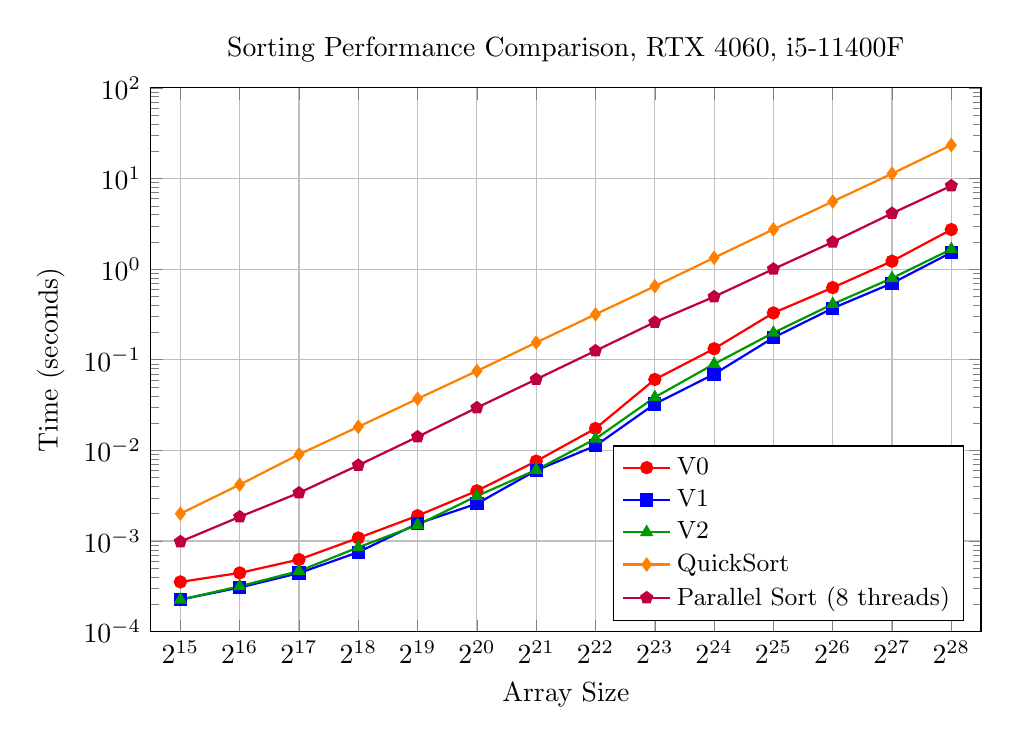
\begin{tikzpicture}
        \begin{semilogyaxis}[
            width=\textwidth,
            height=0.7\textwidth,
            grid=major,
            xlabel={Array Size},
            ylabel={Time (seconds)},
            title={Sorting Performance Comparison, RTX 4060, i5-11400F},
            legend style={
                at={(0.98,0.02)},
                anchor=south east,
                cells={anchor=west},
                font=\small
            },
            xticklabels={$2^{15}$,$2^{16}$,$2^{17}$,$2^{18}$,$2^{19}$,$2^{20}$,$2^{21}$,$2^{22}$,$2^{23}$,$2^{24}$,$2^{25}$,$2^{26}$,$2^{27}$,$2^{28}$},
            xtick={15,16,17,18,19,20,21,22,23,24,25,26,27,28},
            xmin=14.5,
            xmax=28.5,
            ymin=0.0001,
            ymax=100,
            cycle list name=color list
        ]
            % V0 implementation
            \addplot[thick,color=red,mark=*] coordinates {
                (15,0.000354) (16,0.000445) (17,0.000625) (18,0.001081) (19,0.001903)
                (20,0.003582) (21,0.007610) (22,0.017454) (23,0.060665) (24,0.132279)
                (25,0.328798) (26,0.625425) (27,1.223395) (28,2.731731)
            };
            
            % V1 implementation
            \addplot[thick,color=blue,mark=square*] coordinates {
                (15,0.000226) (16,0.000307) (17,0.000443) (18,0.000754) (19,0.001558)
                (20,0.002584) (21,0.006019) (22,0.011254) (23,0.032567) (24,0.069451)
                (25,0.175497) (26,0.370356) (27,0.698480) (28,1.525176)
            };
            
            % V2 implementation
            \addplot[thick,color=green!60!black,mark=triangle*] coordinates {
                (15,0.000225) (16,0.000317) (17,0.000466) (18,0.000852) (19,0.001506)
                (20,0.003140) (21,0.006097) (22,0.013411) (23,0.038572) (24,0.089846)
                (25,0.198383) (26,0.411237) (27,0.794070) (28,1.658931)
            };
            
            % QuickSort Sequential
            \addplot[thick,color=orange,mark=diamond*] coordinates {
                (15,0.002005) (16,0.004188) (17,0.009034) (18,0.018219) (19,0.037159)
                (20,0.075137) (21,0.154943) (22,0.317120) (23,0.647345) (24,1.334878)
                (25,2.747267) (26,5.572010) (27,11.313033) (28,23.412174)
            };
            
            % Parallel Sort
            \addplot[thick,color=purple,mark=pentagon*] coordinates {
                (15,0.000984) (16,0.001850) (17,0.003401) (18,0.006861) (19,0.014129)
                (20,0.029606) (21,0.060891) (22,0.125692) (23,0.259993) (24,0.496197)
                (25,1.002089) (26,1.992052) (27,4.127177) (28,8.313328)
            };
            
            \legend{V0, V1, V2, QuickSort, Parallel Sort (8 threads)}
        \end{semilogyaxis}
    \end{tikzpicture}
    \caption{Performance comparison of different sorting implementations.}
    \label{fig:sorting-performance}
\end{figure}

\begin{figure}[H]
    \centering
    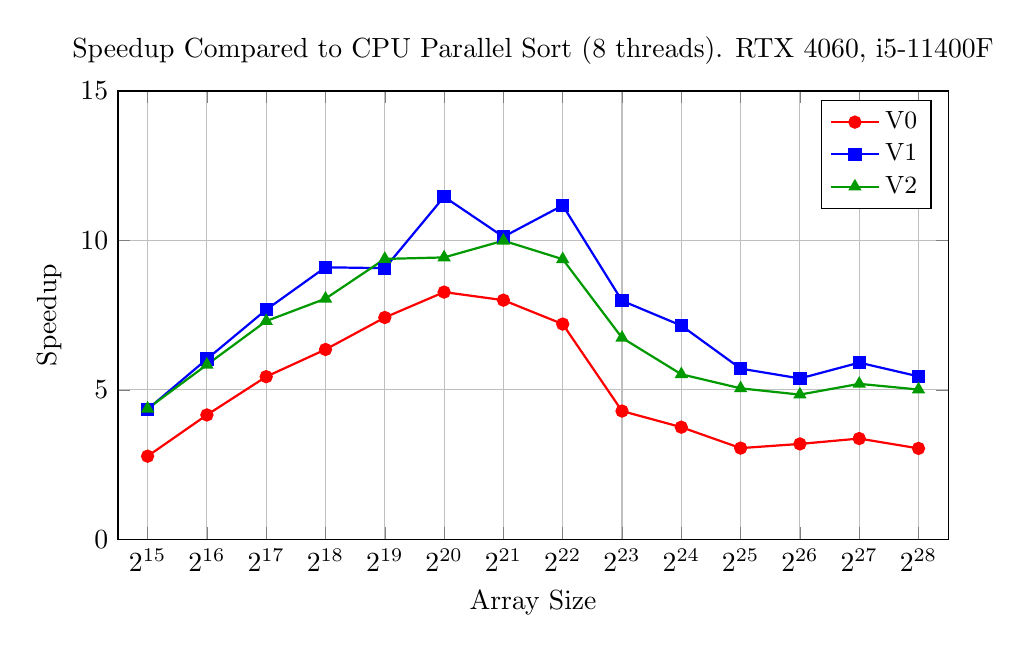
\begin{tikzpicture}
        \begin{axis}[
            width=\textwidth,
            height=0.6\textwidth,
            grid=major,
            xlabel={Array Size},
            ylabel={Speedup},
            title={Speedup Compared to CPU Parallel Sort (8 threads). RTX 4060, i5-11400F},
            legend style={
                at={(0.98,0.98)},
                anchor=north east,
                cells={anchor=west},
                font=\small
            },
            xticklabels={$2^{15}$,$2^{16}$,$2^{17}$,$2^{18}$,$2^{19}$,$2^{20}$,$2^{21}$,$2^{22}$,$2^{23}$,$2^{24}$,$2^{25}$,$2^{26}$,$2^{27}$,$2^{28}$},
            xtick={15,16,17,18,19,20,21,22,23,24,25,26,27,28},
            xmin=14.5,
            xmax=28.5,
            ymin=0,
            ymax=15,
            cycle list name=color list
        ]
            % V0 implementation speedup
            \addplot[thick,color=red,mark=*] coordinates {
                (15,2.78) (16,4.16) (17,5.44) (18,6.35) (19,7.42)
                (20,8.27) (21,8.00) (22,7.20) (23,4.29) (24,3.75)
                (25,3.05) (26,3.19) (27,3.37) (28,3.04)
            };
            
            % V1 implementation speedup
            \addplot[thick,color=blue,mark=square*] coordinates {
                (15,4.35) (16,6.03) (17,7.68) (18,9.10) (19,9.07)
                (20,11.46) (21,10.12) (22,11.17) (23,7.98) (24,7.15)
                (25,5.71) (26,5.38) (27,5.91) (28,5.45)
            };
            
            % V2 implementation speedup
            \addplot[thick,color=green!60!black,mark=triangle*] coordinates {
                (15,4.37) (16,5.84) (17,7.30) (18,8.05) (19,9.38)
                (20,9.43) (21,9.99) (22,9.37) (23,6.74) (24,5.52)
                (25,5.05) (26,4.84) (27,5.20) (28,5.01)
            };
            
            \legend{V0, V1, V2}
        \end{axis}
    \end{tikzpicture}
    \caption{Speedup comparison of GPU implementations relative to CPU parallel sort with 8 threads.}
    \label{fig:speedup-performance}
\end{figure}

\begin{figure}[H]
    \centering
    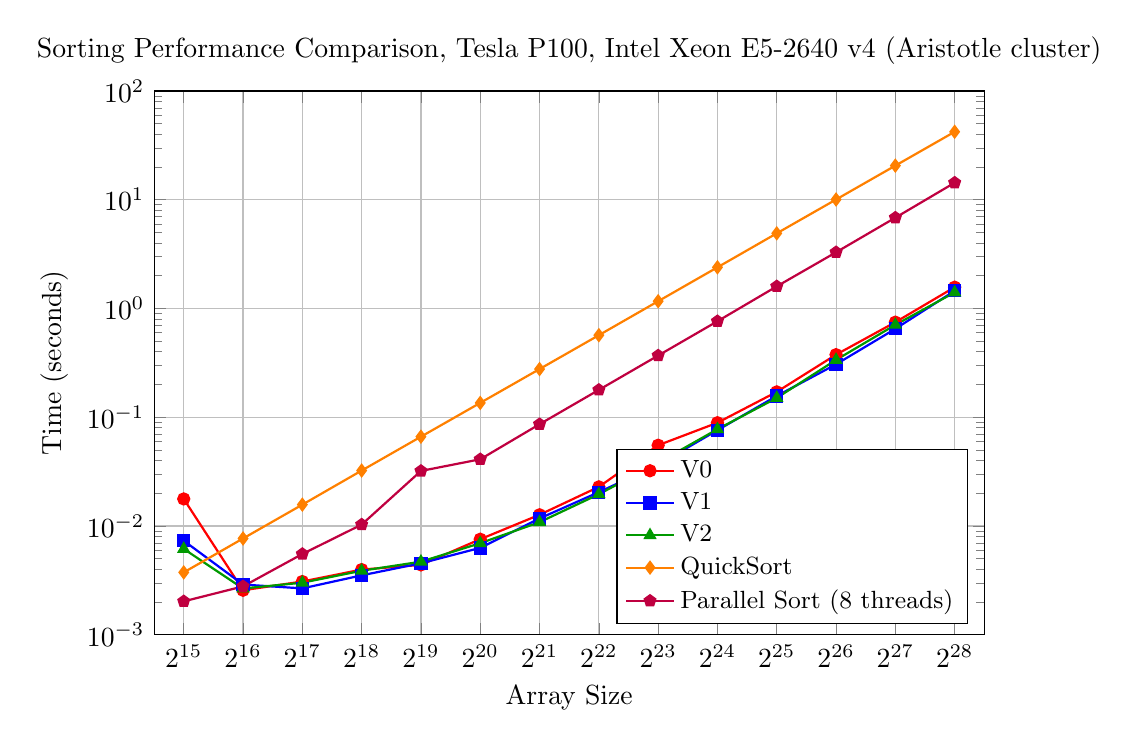
\begin{tikzpicture}
        \begin{semilogyaxis}[
            width=\textwidth,
            height=0.7\textwidth,
            grid=major,
            xlabel={Array Size},
            ylabel={Time (seconds)},
            title={Sorting Performance Comparison, Tesla P100, Intel Xeon E5-2640 v4 (Aristotle cluster)},
            legend style={
                at={(0.98,0.02)},
                anchor=south east,
                cells={anchor=west},
                font=\small
            },
            xticklabels={$2^{15}$,$2^{16}$,$2^{17}$,$2^{18}$,$2^{19}$,$2^{20}$,$2^{21}$,$2^{22}$,$2^{23}$,$2^{24}$,$2^{25}$,$2^{26}$,$2^{27}$,$2^{28}$},
            xtick={15,16,17,18,19,20,21,22,23,24,25,26,27,28},
            xmin=14.5,
            xmax=28.5,
            ymin=0.001,
            ymax=100,
            cycle list name=color list
        ]
            % V0 implementation
            \addplot[thick,color=red,mark=*] coordinates {
                (15,0.017734) (16,0.002564) (17,0.003087) (18,0.003975) (19,0.004388)
                (20,0.007560) (21,0.012682) (22,0.022905) (23,0.055267) (24,0.089043)
                (25,0.171042) (26,0.376266) (27,0.748131) (28,1.568899)
            };
            
            % V1 implementation
            \addplot[thick,color=blue,mark=square*] coordinates {
                (15,0.007321) (16,0.002895) (17,0.002668) (18,0.003517) (19,0.004542)
                (20,0.006293) (21,0.011729) (22,0.020474) (23,0.036630) (24,0.076005)
                (25,0.156914) (26,0.306797) (27,0.650062) (28,1.453431)
            };
            
            % V2 implementation
            \addplot[thick,color=green!60!black,mark=triangle*] coordinates {
                (15,0.006156) (16,0.002664) (17,0.003010) (18,0.003877) (19,0.004696)
                (20,0.006949) (21,0.010843) (22,0.019601) (23,0.038152) (24,0.077626)
                (25,0.150483) (26,0.336624) (27,0.707282) (28,1.405336)
            };
            
            % QuickSort Sequential (unchanged)
            \addplot[thick,color=orange,mark=diamond*] coordinates {
                (15,0.003745) (16,0.007677) (17,0.015713) (18,0.032342) (19,0.066246)
                (20,0.135485) (21,0.277279) (22,0.568027) (23,1.165850) (24,2.389348)
                (25,4.906866) (26,10.043821) (27,20.578749) (28,42.108344)
            };
            
            % Parallel Sort (unchanged)
            \addplot[thick,color=purple,mark=pentagon*] coordinates {
                (15,0.002028) (16,0.002784) (17,0.005527) (18,0.010299) (19,0.032067)
                (20,0.041049) (21,0.086247) (22,0.178383) (23,0.369179) (24,0.763142)
                (25,1.596266) (26,3.285755) (27,6.835703) (28,14.329778)
            };
            
            \legend{V0, V1, V2, QuickSort, Parallel Sort (8 threads)}
        \end{semilogyaxis}
    \end{tikzpicture}
    \caption{Performance comparison of different sorting implementations on Aristotelis cluster.}
    \label{fig:sorting-performance-p100}
\end{figure}

\begin{figure}[H]
    \centering
    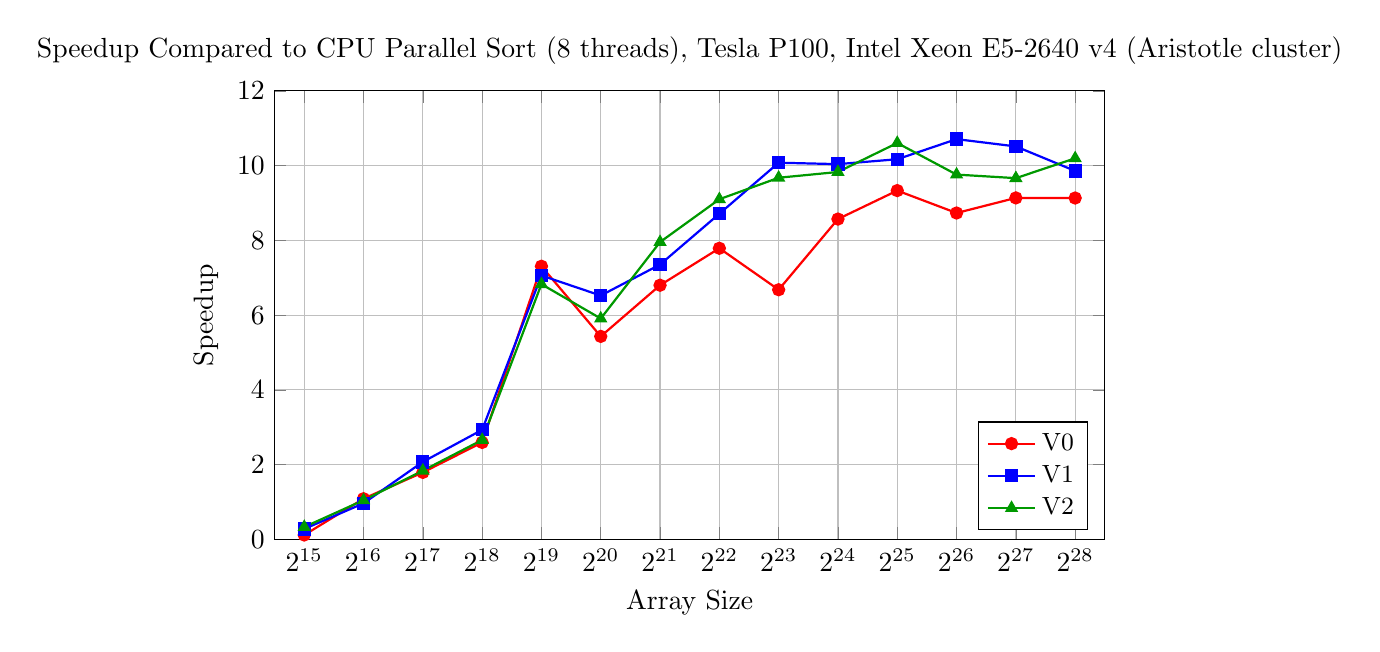
\begin{tikzpicture}
        \begin{axis}[
            width=\textwidth,
            height=0.6\textwidth,
            grid=major,
            xlabel={Array Size},
            ylabel={Speedup},
            title={Speedup Compared to CPU Parallel Sort (8 threads), Tesla P100, Intel Xeon E5-2640 v4 (Aristotle cluster)},
            legend style={
                at={(0.98,0.02)},
                anchor=south east,
                cells={anchor=west},
                font=\small
            },
            xticklabels={$2^{15}$,$2^{16}$,$2^{17}$,$2^{18}$,$2^{19}$,$2^{20}$,$2^{21}$,$2^{22}$,$2^{23}$,$2^{24}$,$2^{25}$,$2^{26}$,$2^{27}$,$2^{28}$},
            xtick={15,16,17,18,19,20,21,22,23,24,25,26,27,28},
            xmin=14.5,
            xmax=28.5,
            ymin=0,
            ymax=12,
            cycle list name=color list
        ]
            % V0 implementation speedup
            \addplot[thick,color=red,mark=*] coordinates {
                (15,0.114) (16,1.086) (17,1.790) (18,2.592) (19,7.308)
                (20,5.430) (21,6.800) (22,7.789) (23,6.679) (24,8.571)
                (25,9.333) (26,8.733) (27,9.137) (28,9.134)
            };
            
            % V1 implementation speedup
            \addplot[thick,color=blue,mark=square*] coordinates {
                (15,0.277) (16,0.962) (17,2.072) (18,2.929) (19,7.060)
                (20,6.523) (21,7.353) (22,8.713) (23,10.079) (24,10.041)
                (25,10.172) (26,10.710) (27,10.515) (28,9.859)
            };
            
            % V2 implementation speedup
            \addplot[thick,color=green!60!black,mark=triangle*] coordinates {
                (15,0.329) (16,1.045) (17,1.837) (18,2.658) (19,6.828)
                (20,5.908) (21,7.955) (22,9.101) (23,9.677) (24,9.831)
                (25,10.607) (26,9.761) (27,9.666) (28,10.197)
            };
            
            \legend{V0, V1, V2}
        \end{axis}
    \end{tikzpicture}
    \caption{Speedup comparison of GPU implementations relative to CPU parallel sort with 8 threads on Aristotelis cluster.}
    \label{fig:speedup-performance-p100}
\end{figure}

In both tests we can see that the V1 implementation is generally the fastest, sometimes surpassed by V2. This result is not
expected since the V2 implementation uses shared memory, which is faster than global memory. However, the synchronizations required
between the threads when transferring the memory could be the reason for the slowdown. A thorough measurement of the execution time 
in each step of the algorithm was performed, with no apparent bottleneck (they can be found on the Github repository). 
Though as expected, the V0 implementation is the slowest.

As for the speedup, we can see that there's a noticeable speed bump compared to a parallel CPU algorithm, indicating that the algorithm
can utilize the GPU resources to sort arrays \textbf{up to 12 times faster}.

\section{Conclusion}
Bitonic sort is a powerful algorithm that can sort large arrays in a parallel manner. By efficiently utilizing the GPU resources
with CUDA, we can achieve a noticeable speedup compared to CPU algorithms. We would expect that the V2 implementation is the fastest,
but further analysis is needed to evaluate the result.

The source code can be found on the \href{https://github.com/NontasBak/CUDA-bitonic-sort}{Github repository}.

\end{document}